\chapter{Machine Learning Models Explored} \label{ChapterMachineLearningModelsExplored}

In this chapter, we investigate which parameters affect the convolutional and dense model's performance for datasets of different complexity. Analyzing which hyperparameters most influence performance informs future research into applying machine learning to gamma-ray spectroscopy. To accomplish this, we ran hyperparameter searches using two datasets: a complete dataset with a wide range of simulated parameters and a simple dataset with smaller parameter ranges. This section describes these datasets and the architectural and regularization hyperparameters choices for the dense and convolutional models. This section concludes with a discussion on the insights obtained from the hyperparameter searches.


% Dense and convolutional models are explored for two different reasons. 

\section{Training Templates Overview}

The datasets used to train the models are created using templates of simulated gamma-ray spectra without Poisson noise. A one-dimensional particle transport code developed at Sandia National Laboratory, GADRAS-DRF (Gamma Detector Response and Analysis Software - Detector Response Function) \cite{mitchell2014}, was used to generate these templates. This simulation code is used to model a radiation detector's response considering environmental scattering and a specific  detector's properties. The GADRAS-DRF interface in Figure \ref{fig:gadras_parameters} shows the detector parameters used in this work. These parameters are from an Ortec 905-3 NaI(Tl) detector included in the Department of Homeland Security's Algorithm Improvement Program (AIP) software package \cite{DHSAIP}. To simulate our template spectra, the detector model's default energy calibration was modified so the detector measured energies from 0 MeV to 3.5 MeV. This was accomplished by setting the calibration offset (Order 0 in E) to zero and the calibration's gain (Order 1 in E) to 3500. The default number of channels was also changed to 1194, calibrating the 1024$^{th}$ channel - the default spectrum length used in this work - to an energy of 3 MeV. This ensures that isotopic signatures higher than 3 MeV are included in the training dataset when a template's calibration is modified to include these energies.

\begin{figure}[H]
	\centering
	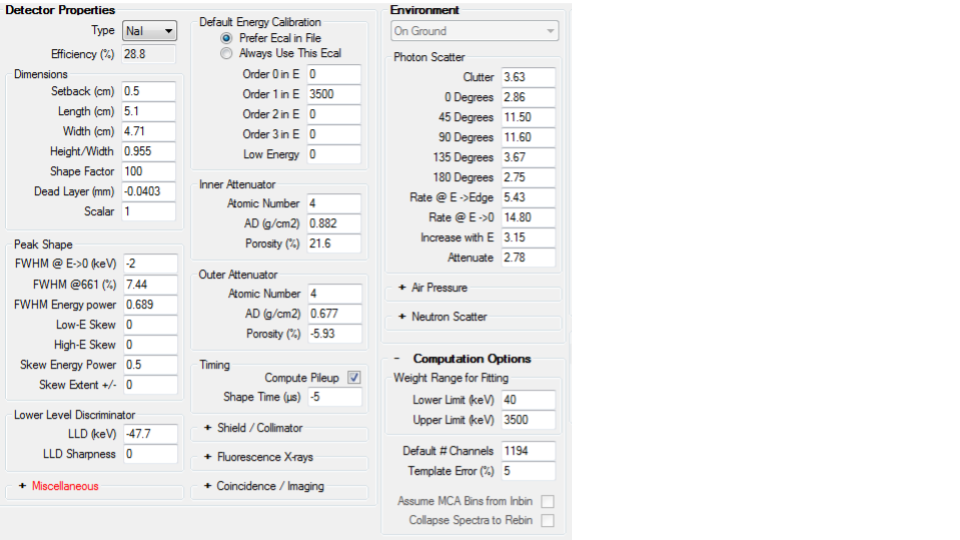
\includegraphics[trim=0 0 390 0,clip,width=0.7\linewidth]{images/gadras_parameters}
	\caption{GADRAS-DRF GUI showing parameters used to simulate the Ortec 905-3 2x2-in NaI(Tl) detector used in this work.}
	\label{fig:gadras_parameters}
\end{figure}


GADRAS-DRF was also used to simulate spectral changes associated with measurement geometry. The measurement scenario used by GADRAS-DRF is illustrated in Figure \ref{fig:gadras_measurement_setup}. Using GADRAS-DRF, we can simulate changes in source-detector distance, the source and detector's mutual height from the ground, and optional shielding material between the source and detector. To demonstrate two of these effects, $^{60}$Co spectra were simulated at various source-detector distances, Figure \ref{fig:sim_spectra_distance_comparison}, and heights ground, Figure \ref{fig:sim_spectra_height_comparison}. These parameters change the Compton continuum's shape, the peak-to-total ratio, and the backscatter peak's magnitude. Another parameter that changes the spectrum is the Gaussian energy broadening of the photopeaks. Due to manufacturing differences, each detector has a different amount of energy broadening. Examples of $^{60}$Co spectra with different FWHM parameters are shown in Figure \ref{fig:sim_spectra_FWHM_comparison}.


\begin{figure}[H]
	\centering
	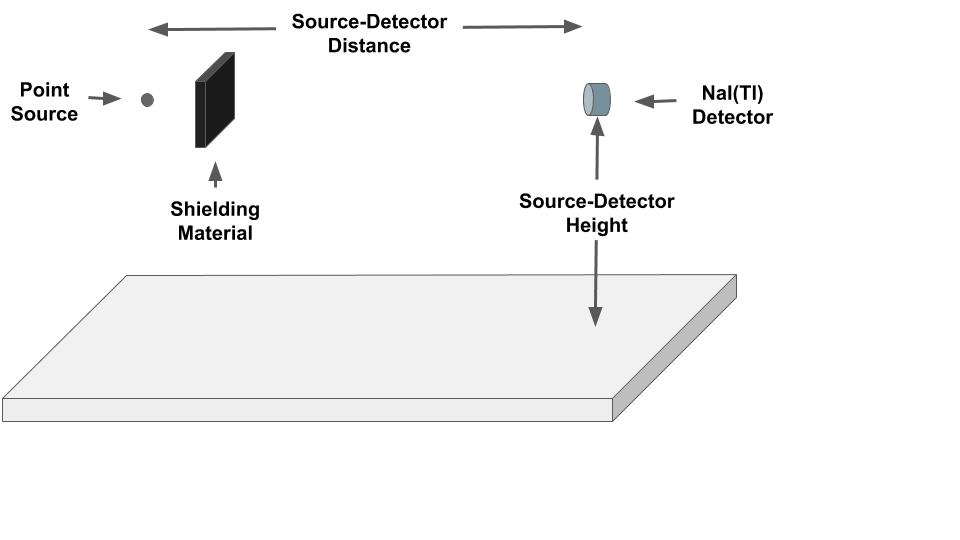
\includegraphics[trim=0 0 180 0,clip,width=0.9\linewidth]{images/gadras_measurement_setup}
	\caption{GADRAS-DRF measurement diagram. Environmental scatter is approximated using the photon scatter terms from Figure \ref{fig:gadras_parameters}.}
	\label{fig:gadras_measurement_setup}
\end{figure}



\begin{figure}[H]
\centering
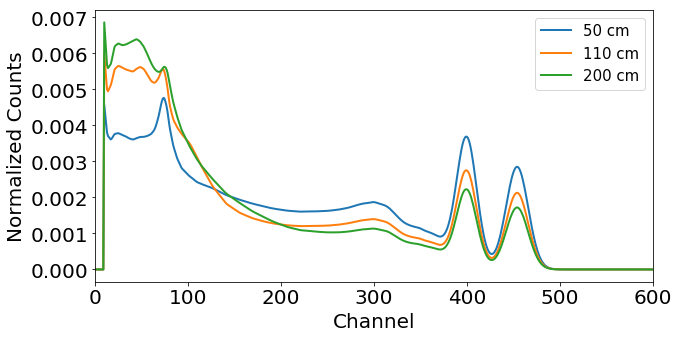
\includegraphics[width=0.75\linewidth]{images/sim_spectra_distance_comparison}
\caption{Comparison of a $^{60}$Co spectrum simulated using various source-detector distances.}
\label{fig:sim_spectra_distance_comparison}
\end{figure}

\begin{figure}[H]
\centering
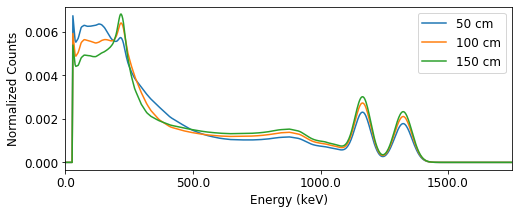
\includegraphics[width=0.75\linewidth]{images/sim_spectra_height_comparison}
\caption{Comparison of a $^{60}$Co spectrum simulated using various source-detector heights off the ground.}
\label{fig:sim_spectra_height_comparison}
\end{figure}


\begin{figure}[H]
\centering
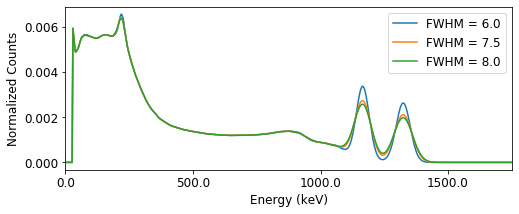
\includegraphics[width=0.75\linewidth]{images/sim_spectra_FWHM_comparison}
\caption{Comparison of a $^{60}$Co spectrum simulated with various FWHM parameters.}
\label{fig:sim_spectra_FWHM_comparison}
\end{figure}




% To incorporate these changes, templates simulated at different distances are included in the dataset. These distances start at 30cm, which is the distance at which a 1 uCi source will have an activity of about 400 cps on a 2 inch diameter detector. This is about twice the expected activity of background. 

% Changes in calibration due to temperature shifts are also considered. Due to the relatively large magnitude in calibration shifts due to temperature shifts from -5 C to 40 C \cite{CASANOVAS2012588}, it is expected incorporating these additions will also make the algorithm robust against calibration.

The template parameters used in this study are shown in Table \ref{table:all_fixed_simulation_parameters}. These parameters are based on handheld RIID scenarios. The source-detector height off the ground are sampled between shin and arm heights (50 cm to 150 cm). The source-detector distance range corresponds to standoff distances expected when measuring a source in a cargo container. The areal density of each material corresponds to 20$\%$, 40$\%$, 60$\%$, and 80$\%$ attenuation of a 200 keV photon. This photon energy was chosen because it is near the 186 keV energy of the characteristic $^{235}$U photopeak. A set of unshielded templates is also included. The FWHM range was chosen based on reported FWHM values for a NaI(Tl) detector (see section \ref{subsection_energy_resolution}). Background locations were chosen based on their geographic and geologic differences.

\begin{table}[H]
	\centering
	\caption{Fixed GADRAS-DRF template simulation parameters.}
	\begin{tabular}{ll}
		\hline
		\textbf{Simulation Parameter} & \textbf{Values} \\ \hline
		source-detector height [cm] & 50, 100, 125 \\ 
		source-detector distance [cm] & 50, 175, 300 \\ 
		Areal density of solid aluminum [$\frac{\text{g}}{\text{cm}^{2}}$] & 1.82, 4.18, 7.49, 13.16 \\ 
		Areal density of solid iron [$\frac{\text{g}}{\text{cm}^{2}}$] & 1.53, 3.5, 6.28, 11.02 \\ 
		Areal density of solid lead [$\frac{\text{g}}{\text{cm}^{2}}$] & 0.22, 0.51, 0.92, 1.61 \\ 
		FWHM at  662 keV [\%] & 7.0, 7.5, 8.0 \\ 
		Background Location & \begin{tabular}[l]{@{}l@{}}Albuquerque, Atlanta, Austin,\\ Chicago , Knoxville , Miami\end{tabular} \\ \hline
	\end{tabular}
	\label{table:all_fixed_simulation_parameters}
\end{table}

In addition to the parameters simulated by GADRAS-DRF, parameters are included to perform additional data augmentation. These parameters are shown in Table \ref{table:all_variable_simulation_parameters}.

\begin{table}[H]
\centering
\caption{Default data augmentation parameters.}
\begin{tabular}{l}
\hline
\textbf{Simulation Parameter} \\ \hline
integration time \\ 
background counts per second \\ 
Signal to Background ratio \\ 
Calibration - Offset \\ 
Calibration - Gain \\ \hline
\end{tabular}
\label{table:all_variable_simulation_parameters}
\end{table}

\section{Hyperparameter Search}

To determine which parameters affect the convolutional and dense model's performance on datasets of increasing complexity, hyperparameter searches for each model are performed for a simple and more complicated dataset. The hyperparameter search for a single model and dataset is illustrated in Figure \ref{fig:hyperparameter_search_workflow}. For each dataset and model, 5-folds cross validation is performed on 256 sets of randomly chosen hyperparameters. The maximum number of epochs was set to 200 and an early stopping patience of 20 epochs was used to stop training with the validation dataset's F1 score. In addition to this, training was ended after 10 epochs if the validation dataset's F1 score did cross a 10\% threshold. The hyperparameter combination with the lowest average validation dataset F1 score was declared the optimum hyperparameter combination for that model. The validation dataset being used to end training induces a biased into the score used to determine the best hyperparameter combination. A better approach would be to use the a separate testing dataset's F1 score to determine the optimum hyperparameter combination.

\begin{figure}[H]
	\centering
	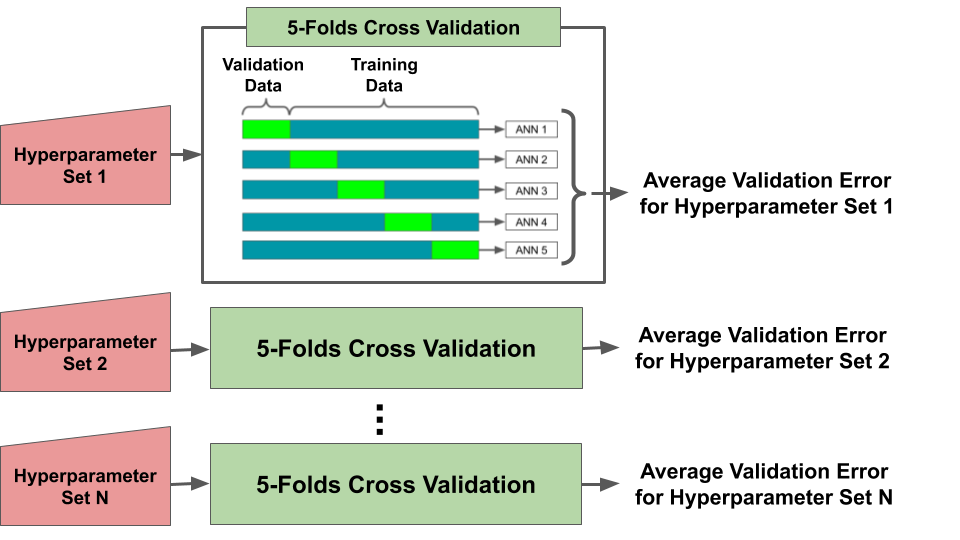
\includegraphics[trim=0 0 40 0,clip,width=1.0\linewidth]{images/hyperparameter_search_workflow}
	\caption{Hyperparameter search workflow.}
	\label{fig:hyperparameter_search_workflow}
\end{figure}


\section{Datasets Used for the Hyperparameter Search} \label{datasets_used_hyperparam_search}

The parameters used for the simple dataset are shown in Table \ref{table:hyperparameter_dataset_easy_parameters} and parameters used for the complete dataset are shown in Table \ref{table:hyperparameter_dataset_full_parameters}. Datasets are simulated using the process described in Section \ref{section_dataset_gen}. Isotopes included in the dataset are from the  ANSI N42-34-2006 standard for isotope identification devices \cite{ANSI}: $^{241}$Am, $^{133}$Ba, $^{57}$Co, $^{60}$Co, $^{51}$Cr, $^{137}$Cs, $^{152}$Eu, $^{67}$Ga, $^{123}$I, $^{125}$I, $^{131}$I, $^{111}$In, $^{192}$Ir, $^{177m}$Lu, $^{99}$Mo, $^{237}$Np, $^{103}$Pd, $^{239}$Pu, $^{240}$Pu, $^{226}$Ra, $^{75}$Se, $^{153}$Sm, $^{99m}$Tc, $^{201}$Tl, $^{204}$Tl, $^{233}$U, $^{235}$U, $^{238}$U, and $^{133}$Xe. In each dataset, a total of 100 spectra were simulated for each isotope. Each dataset also included 100 spectra of only background.

\begin{table}[H]
	\centering
	\caption{Range of parameters used for the simple dataset.}
	\label{table:hyperparameter_dataset_easy_parameters}
	\begin{tabular}{lll}
		\hline
		\textbf{Simulation Parameter} & \textbf{Parameter Range} & \textbf{Sampling} \\ \hline
		Source-Detector Distance [cm] & 175 & N/A \\ 
		Source-Detector Height [cm] & 100 & N/A \\ 
		FWHM at 662 keV & 7.5 & N/A \\ 
		Shielding [\% 200 keV Attenuated] & 0\%, 20\% & Uniform \\ 
		Integration Time [s] & 60 - 600 & Log-Uniform \\ 
		Calibration - Offset [channels] & 0 - 10 & Uniform \\ 
		Calibration - Gain & 0.9 - 1.1 & Uniform \\ 
		Signal to Background Ratio & 0.5 - 2.0 & Uniform \\ 
		Background Counts Per Second & 200 & Poisson \\ \hline
	\end{tabular}
\end{table}


\begin{table}[H]
	\centering
	\caption{Range of parameters used for the complete dataset.}
	\label{table:hyperparameter_dataset_full_parameters}
	\begin{tabular}{lll}
		\hline
		\textbf{Simulation Parameter} & \textbf{Parameter Range} & \textbf{Sampling} \\ \hline
		Source-Detector Distance {[}cm{]} & 50, 175, 300 & Uniform \\ 
		Source-Detector Height {[}cm{]} & 50, 100, 150 & Uniform \\ 
		FWHM 662 keV {[}s{]} & 7.0, 7.5, 8.0 & Uniform \\ 
		Shielding [\% 200 keV Attenuated] & 0\%, 20\%, 40\%, 60\% & Uniform \\ 
		Integration Time {[}s{]} & 10 - 3600 & Log-Uniform \\ 
		Calibration - Offset (channels) & 0 - 10 & Uniform \\ 
		Calibration - Gain & 0.8 - 1.2 & Uniform \\ 
		Signal to Background Ratio & 0.1 - 3.0 & Uniform \\ 
		Background Counts Per Second & 200 & Poisson \\ \hline
	\end{tabular}
\end{table}


The hyperparameter search for a single model and dataset is illustrated in Figure \ref{fig:hyperparameter_search_workflow}. For each dataset and model, 5-folds cross validation is performed on 256 sets of randomly chosen hyperparameters. The maximum number of epochs was set to 200 and an early stopping patience of 20 epochs was used to stop training using the validation dataset's F1 score,
%
\begin{align} \label{eq:f1_score}
\text{F1 score} &= 2 \frac{\text{precision} \cdot \text{recall}}{\text{precision + recall}} \\
\text{where precision} &= \frac{\text{true positives}}{\text{true positives + false positives}} \nonumber \\
\text{recall} &= \frac{\text{true positives}}{\text{true positives + false negatives}}. \nonumber \\
\end{align}
%
In addition to this, training was ended after 10 epochs if the validation dataset's F1 score did cross a 10\% threshold. The hyperparameter combination with the lowest average validation dataset F1 score was declared the optimum hyperparameter combination for that model. The validation dataset being used to end training induces a biased into the score used to determine the best hyperparameter combination. A better approach would be to use a separate simulated dataset's F1 score to determine the optimum hyperparameter combination.

\begin{figure}[H]
	\centering
	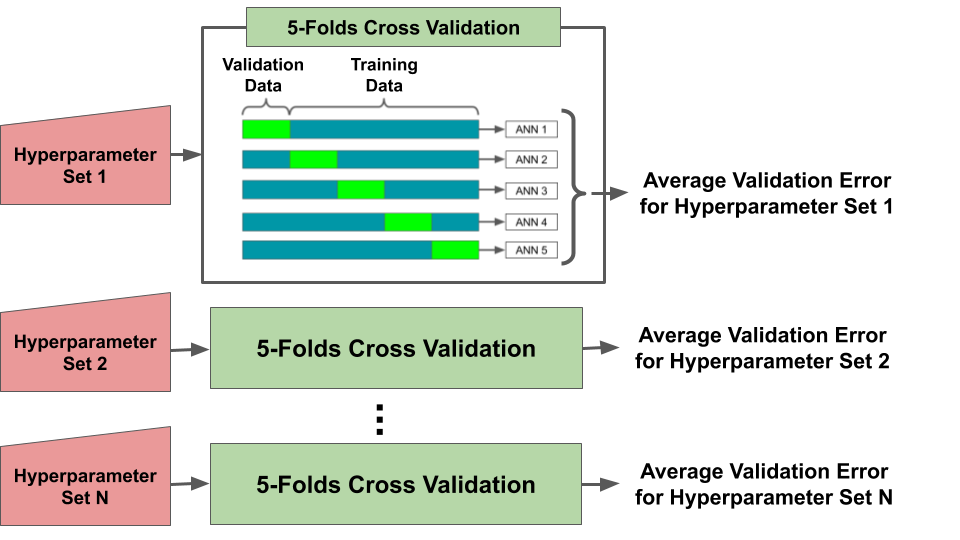
\includegraphics[trim=0 0 40 0,clip,width=1.0\linewidth]{images/hyperparameter_search_workflow}
	\caption{Hyperparameter search workflow.}
	\label{fig:hyperparameter_search_workflow}
\end{figure}

\section{Hyperparameter Search Results}

In this section, hyperparameter search results are shown using random efficiency curves and by comparing parameter values versus average validation set F1 scores from the 5-fold cross validation. Random efficiency experiment curves indicate the quality of the hyperparameter search space and allow for reproducibility. Analyzing how the parameter values change the F1 score indicates which parameters are important. Hyperparameter bounds are based on previous published experiments as well as literature recommendations \cite{kamuda2017, kamuda2018, Bengio2018}.

% A sharper efficiency curve shows that many hyperparameter combinations perform well, whereas 

% The shape of this curve indicates the frequency of good models under random search, and quantifies the relative volumes (in search space) of the various levels of performance - Bergstra2012a


% These also allow for researchers who want to fit models to this dataset to have a performance benchmark. If you wanted to compare random hyperparameter search to more intelligent methods, you could compare using this.

\subsection{Dense Architecture}

The architecture and training hyperparameters used to construct DNN's are shown in Table \ref{table:hyperparameter_dataset_parameters_DNN}. The number of densely connected nodes decreases for each subsequent layer. The input scaling is read left-to-right. For example, the $sqrt-max$ scaling would first take the square root of the each channel in the spectrum and then normalized the spectrum by its maximum value. The $L1-norm$ normalizes a spectrum by its L1 norm. The $log1p$ function is defined as 
\begin{align} \label{eq:single_layer_eq_sum}
log1p(x) := log_{10}(x+1)
\end{align}

\begin{table}[H]
\centering
\caption{Range of hyperparameters explored for the DNN.}
\label{table:hyperparameter_dataset_parameters_DNN}
\begin{tabular}{lll}
\hline
\textbf{Hyperparameter} & \textbf{Hyperparameter Range} & \textbf{Sampling} \\ \hline
Number of Layers & 1 - 3 & Uniform \\
Nodes in Layer & 32, 64, 128, 256, 512 & Uniform \\
Initial Learning Rate & 10$^{-4}$ - 10$^{-1}$ & Log-Uniform \\
L2 Regularization Strength & 10$^{-2}$ - 10$^{0}$ & Log-Uniform \\
Dropout Frequency & 0 - 1 & Uniform \\
Batch Size & 16, 32, 64, 128, 256, 512 & Uniform \\
Activation Function & relu, tanh & Uniform \\
Input Scaling & \begin{tabular}[l]{@{}l@{}}sqrt \\ sqrt-max \\ sqrt-L1 norm \\ log1p \\ log1p-max \\ log1p-L1 norm\end{tabular} & Uniform \\ \hline
\end{tabular}
\end{table}



Random efficiency experiment curves for the DNN trained on the simple and complete datasets are shown in Figures \ref{fig:random_hp_search_dnn_easy} and \ref{fig:random_hp_search_dnn_full}. A large number of hyperparameter combinations did not reduce the validation dataset's F1 score above the 10\% threshold after 10 epochs, ending their training early. As expected, the complete dataset took more trials to obtain good performance. The median validation dataset's F1 score in the simple dataset begins to asymptote after an experiment size of 16 while the validation dataset's F1 score in the complete dataset does not asymptote. This indicated that when applying DNN's to more difficult problems in gamma-ray spectroscopy either wider hyperparameter ranges need to be explored, more advanced hyperparameter search strategies need to be employed, or that due to their structure DNN's are not well suited to perform tasks in gamma-ray spectroscopy.

\begin{figure}[H]
	\centering
	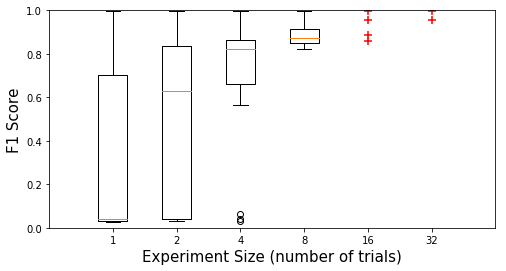
\includegraphics[width=0.8\linewidth]{images/random_hp_search_dnn_easy}
	\caption{Random hyperparameter search efficiency curves for the DNN using the simple dataset.}
	\label{fig:random_hp_search_dnn_easy}
\end{figure}

\begin{figure}[H]
	\centering
	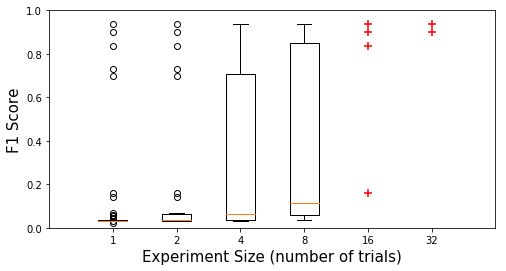
\includegraphics[width=0.8\linewidth]{images/random_hp_search_dnn_full}
	\caption{Random hyperparameter search efficiency curves for the DNN using the complete dataset.}
	\label{fig:random_hp_search_dnn_full}
\end{figure}


Figure \ref{fig:dense_hyperparameters_f1_score} shows the distribution of average validation dataset F1 score from the 5-folds cross validation for each hyperparameter. Conclusions based on these will suffer from a small sample size because few networks trained on the complete dataset achieved high validation dataset F1 scores. General trends in the simple dataset are more representative of actual hyperparameter performance compared to the complete dataset.

Sub-figure \ref{fig:dnn_learning_rate} shows that a learning rate less than 10$^{-2}$ should be used when conducting hyperparameter searches for spectroscopic datasets of similar complexity. This figure also shows that the complete dataset prefers a slower learning rate, with best performing networks using learning rates below 10$^{-3.5}$. Smaller learning rates should also be explored in future searches, if computationally feasible.

Sub-figure \ref{fig:dnn_dropout} shows that the dropout rate has a less obvious performance cutoff compared to the learning rate. This is likely because the dropout value does not have a large effect on training.

Sub-figure \ref{fig:dnn_batch_size} shows that the simple dataset works well in a variety of mini-batch sizes, while the complete dataset may require a larger mini-batch size.

Sub-figures \ref{fig:dnn_dense_nodes_total} and \ref{fig:dnn_dense_layers_total} show the effect of model capacity on performance. Model capacity is comparable to the number of free parameters of a model; too much capacity can lead to overfitting and too little capacity may be insufficient to fit complex data. Overfitting can be seen in the performance drop in three dense layers. Additional layers are unnecessary for problems of this difficulty with the hyperparameters explored. For the complete dataset a significant number of networks perform well with a total number of nodes between 250 and 1000. The simple dataset performed well with a wide range of total nodes.

Sub-figures \ref{fig:dnn_scaler} shows the effect of feature preprocessing on performance. L1 normalization performs very poorly due to the numerical scale of the features. Gradients computed with learning rates explored by the hyperparameter search are too small to significantly update the weights because the features are on the order 10$^{-3}$. Features explored by the other methods are typically between 10$^{0}$ - 10$^{2}$. Scaling spectra using the $sqrt$ of their features makes networks perform well for both datasets. In particular, using $sqrt-max$ scaling produces the most models with high validation dataset F1 scores.

\newcommand{\bluecircle}{\raisebox{2pt}{\tikz{\filldraw[color=blue!60, fill=blue!60, very thick] circle (1.5mm);}}}
\definecolor{darkgreen}{rgb}{0,0.3,0}

\begin{figure}[H]
     \centering
     \begin{subfigure}[b]{0.49\textwidth}
         \centering
         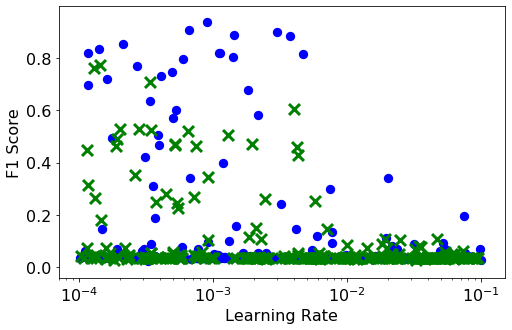
\includegraphics[width=\textwidth]{images/dnn_learning_rate.png}
         \caption{}
         \label{fig:dnn_learning_rate}
     \end{subfigure}
     \hfill
     \begin{subfigure}[b]{0.49\textwidth}
         \centering
         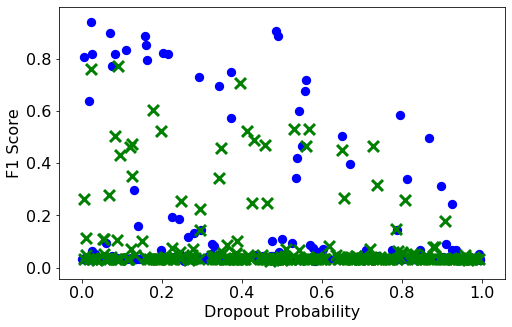
\includegraphics[width=\textwidth]{images/dnn_dropout.png}
         \caption{}
         \label{fig:dnn_dropout}
     \end{subfigure}

     \begin{subfigure}[b]{0.49\textwidth}
         \centering
         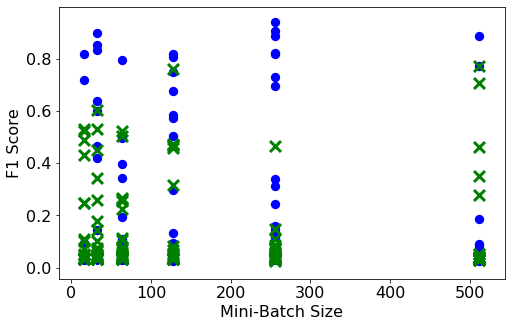
\includegraphics[width=\textwidth]{images/dnn_batch_size.png}
         \caption{}
         \label{fig:dnn_batch_size}
     \end{subfigure}
     \hfill
     \begin{subfigure}[b]{0.49\textwidth}
         \centering
         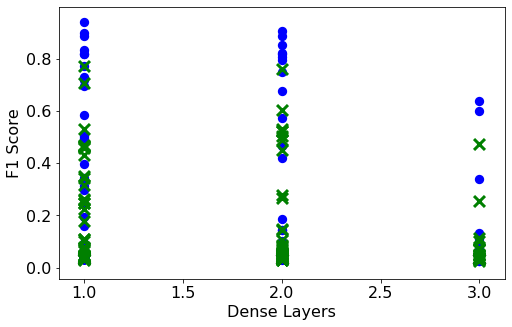
\includegraphics[width=\textwidth]{images/dnn_dense_layers_total.png}
         \caption{}
         \label{fig:dnn_dense_layers_total}
     \end{subfigure}

    \begin{subfigure}[b]{0.49\textwidth}
         \centering
         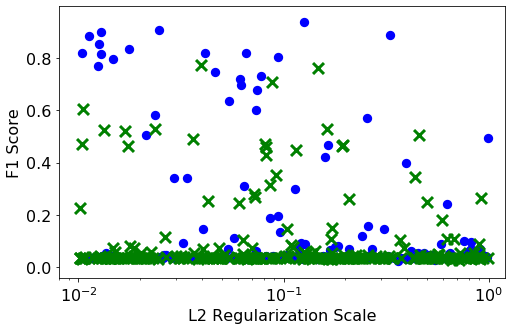
\includegraphics[width=\textwidth]{images/dnn_l2_reg.png}
         \caption{}
         \label{fig:dnn_l2_reg}
     \end{subfigure}
     \hfill
     \begin{subfigure}[b]{0.49\textwidth}
         \centering
         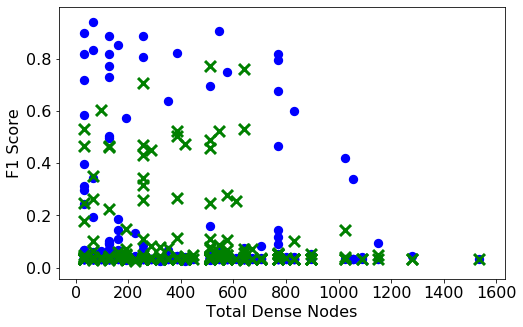
\includegraphics[width=\textwidth]{images/dnn_dense_nodes_total.png}
         \caption{}
         \label{fig:dnn_dense_nodes_total}
     \end{subfigure}     

    \begin{subfigure}[b]{0.49\textwidth}
        \centering
        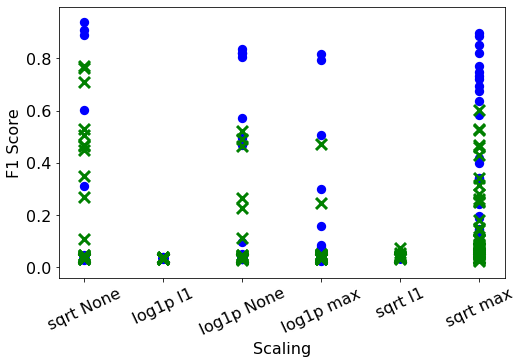
\includegraphics[width=\textwidth]{images/dnn_scaler.png}
         \caption{}
        \label{fig:dnn_scaler}
    \end{subfigure}
    \hfill
    \begin{subfigure}[b]{0.49\textwidth}
        \centering
        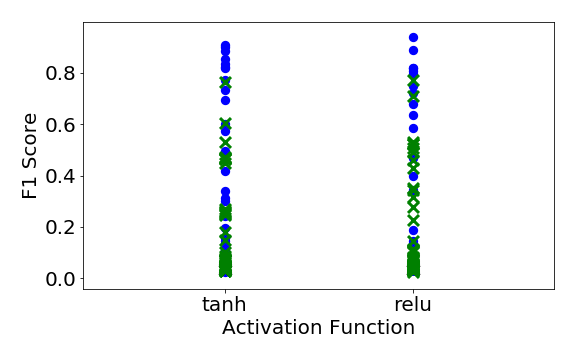
\includegraphics[width=\textwidth]{images/dnn_activation_function.png}
         \caption{}
        \label{fig:dnn_activation_function}
    \end{subfigure}
        \begin{tabular}{r@{ : }l r@{ : }l}
			\textcolor{darkgreen}{\textbf{\large{X}}} & Complete Dataset & \bluecircle & Simple Dataset \\
		\end{tabular}
        \caption{Effect of dense hyperparameters on the validation dataset's final F1 score.}
        \label{fig:dense_hyperparameters_f1_score}
\end{figure}


% \subsubsection{Hyperparameter Search Results - Autoencoders}

% Now that we know optimized autoencoder architectures for the DNN, we need to optimize training hyperparameters. 

% https://machinelearningmastery.com/activation-regularization-for-reducing-generalization-error-in-deep-learning-neural-networks/

% \cite{Ranzato2007} Fig 6 shows you can freeze the unsupervised feature extraction network and update the classifier if you have enough data.

% Sparse denoising autoencoders are included in in this work as feature extraction and dimension reduction techniques. Both autoencoders employ regularization techniques to ensure useful representations are learned. Both models includes $l1$ activity regularization as a method to induce sparsity on the networks activations, which increases generalization \cite{Goodfellow-et-al-2016}. 

% Show how well autoencoders worked at spectrum reconstruction and background subtraction. See if there's a large difference between doing background subtraction and 
\begin{table}[H]
\centering
\caption{Optimum DNN hyperparameter combination found for the simple and complete dataset.}
\label{table:hyperparameter_opt_parameters_DNN}
\begin{tabular}{lll}
\hline
\multirow{2}{*}{\textbf{Hyperparameter}} & \multicolumn{2}{l}{\textbf{Optimum Value}} \\
 & \textbf{Simple Dataset} & \textbf{Complete Dataset} \\ \hline
Dense Layer Hidden Nodes & 64 & 32 \\
Initial Learning Rate & 0.00089 & 0.00024 \\
L2 Regularization Strength & 0.13 & 0.0097 \\
Dropout Frequency & 0.023 & 0.16 \\
Batch Size & 256 & 16 \\
Activation Function & relu & relu \\
Input Scaling & sqrt & sqrt-max \\ 
Total Trainable Weights & 67550 & 540190 \\ \hline
\end{tabular}
\end{table}





\subsection{Convolution Architecture}

The architecture and training hyperparameters used to construct CNN's are shown in Table \ref{table:hyperparameter_dataset_parameters_CNN}. Note, as with the DNN the number of densely connected nodes decreased with each subsequent layer. A smaller range of batch sizes was searched in the CNN compared to the DNN due to computational constraints.

\begin{table}[H]
\centering
\caption{Range of hyperparameters explored for the CNN.}
\label{table:hyperparameter_dataset_parameters_CNN}
\begin{tabular}{lll}
\hline
\textbf{Hyperparameter} & \textbf{Hyperparameter Range} & \textbf{Sampling} \\ \hline
Filter Kernels in Each Layer& \begin{tabular}[l]{@{}l@{}} 4 \\ 8 \\ 16 \\ 32 \\ 4 - 8 \\ 8 - 16 \\ 16 - 32 \\ 4 - 8 - 16 \\  8 - 16 - 32 \end{tabular} & Uniform \\
Filter Kernel Lengths & 2, 4, 8, 16 & Uniform \\
Pooling size & 2, 4, 8, 16 & Uniform \\
Number of Dense Layers & 1 - 3 & Uniform \\
Nodes in Dense Layers & 10 - 1000 & Log-Uniform \\
Initial Learning Rate & 10$^{-4}$ - 10$^{-1}$ & Log-Uniform \\
L2 Regularization Strength & 10$^{-3}$ - 10$^{0}$ & Log-Uniform \\
Dropout Frequency & 0 - 1 & Uniform \\
Batch Size & 16, 32 & Uniform \\
Activation Function & tanh, relu & Uniform \\
Input Scaling & \begin{tabular}[l]{@{}l@{}}sqrt \\ sqrt-max \\ sqrt-L1 norm \\ log1p \\ log1p-max \\ log1p-L1 norm\end{tabular} & Uniform \\ \hline
\end{tabular}
\end{table}


Random efficiency experiment curves for the CNN trained on the simple and complete datasets are shown in Figures \ref{fig:random_hp_search_cnn_easy} and \ref{fig:random_hp_search_cnn_full}. Similar to the dense network, a large number of hyperparameter combinations did not reduce their validation dataset's F1 score in the training set in enough epochs and their training was ended early. Contrary to the DNN, the median validation dataset's F1 score in both datasets smoothly increased with additional trials. Both datasets achieved validation dataset F1 scores above 90$\%$. This demonstrates that the hyperparameter bounds used for both problems are well suited to the problems and that the CNN architectures explored in this search have more potential than the DNN architectures for gamma-ray spectroscopy. As with the DNN, validation dataset F1 scores on the simple dataset are higher than the validation dataset F1 scores on the complete dataset.

\begin{figure}[H]
	\centering
	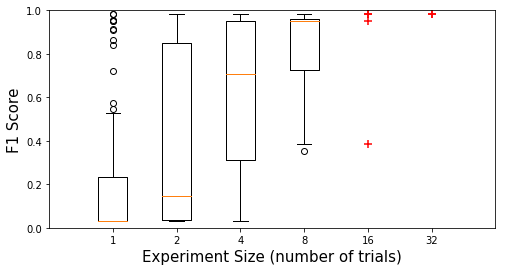
\includegraphics[width=0.8\linewidth]{images/random_hp_search_cnn_easy}
	\caption{Random hyperparameter search efficiency curves for the CNN using the simple dataset.}
	\label{fig:random_hp_search_cnn_easy}
\end{figure}

\begin{figure}[H]
	\centering
	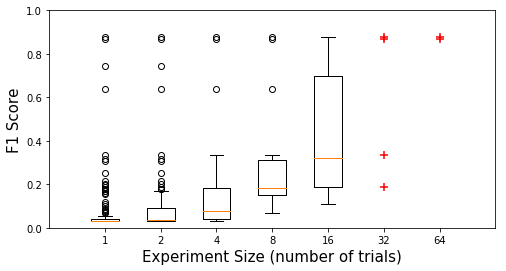
\includegraphics[width=0.8\linewidth]{images/random_hp_search_cnn_full}
	\caption{Random hyperparameter search efficiency curves for the CNN using the complete dataset.}
	\label{fig:random_hp_search_cnn_full}
\end{figure}


Figure \ref{fig:cnn_hyperparameters_f1_score} shows the distribution of hyperparameters searched for the CNN and their average validation dataset F1 scores from the 5-folds cross validation. Similar to the DNN, few networks trained on the complete dataset achieved high validation dataset F1 scores. Conclusions based on these diagrams suffer from a small (albeit larger than the DNN) sample size.

The CNN's training performance is largely agnostic to many hyperparameters, including those associated with the dense part of the CNN. Figure \ref{fig:cnn_hyperparameters_f1_score} shows that both datasets train similarly over a wide range of learning rates below 10$^{-2}$, dense layer dropout rates below 0.8, L2 regularization scales below 10$^{-1}$, between 50 - 200 total dense nodes, and both mini-batch sizes.

The CNN's training performance on the complete dataset is sensitive to hyperparameters related to model capacity. The total number of convolutional layers have the largest affect on the performance of models trained using the complete dataset. Because of the additional complexity in the complete dataset, deeper networks - which extract more abstract features - are necessary for good performance. CNNs with additional convolutional layers should be explored for problems of similar complexity. Additional dense layers did not provide the same boost in performance. Models trained using the simple dataset perform well with a large range of total dense layers while the complete dataset performs well with fewer layers, achieving the best validation dataset F1 score with a two layers. Simple and complete models with three dense layers have maximum F1 scores lower than two or three dense layers.

Performance is also sensitive to other convolutional hyperparameters. Models trained using the simple datasets perform well with each convolutional pooling size. As a general trend, models trained with the complete dataset perform better with larger convolutional pooling sizes. Longer pooling sizes add more shift and scale invariance, which is more important in the complete dataset due to a wider range of detector gain settings. Longer pooling sizes are necessary to incorporate photopeaks and Compton continua, where smaller pooling sizes may be sufficient to retain only photopeak information. Identifying the photopeaks may be enough to identify isotopes in the simple dataset because there are fewer confounding variables. Convolutional kernel lengths of 16 are required for optimal performance for both datasets. The preference for depth in the convolutional part of the CNN is also seen in the number of convolutional filters.

The effect of scaling on performance was similar to the DNN. Using $sqrt$ scaling yielded the best performing networks, especially when tied with $max$ normalization.


\begin{figure}[H]
     \centering
     \begin{subfigure}[b]{0.49\textwidth}
         \centering
         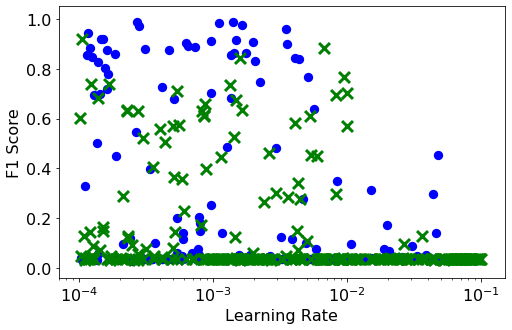
\includegraphics[width=\textwidth]{images/cnn_learning_rate.png}
         \caption{}
         \label{fig:cnn_learning_rate}
     \end{subfigure}
     \hfill
     \begin{subfigure}[b]{0.49\textwidth}
         \centering
         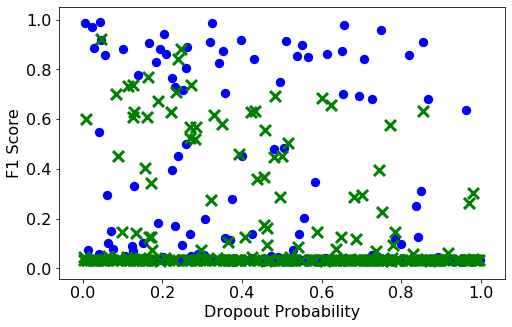
\includegraphics[width=\textwidth]{images/cnn_dropout.png}
         \caption{}
         \label{fig:cnn_dropout}
     \end{subfigure}

     \begin{subfigure}[b]{0.49\textwidth}
         \centering
         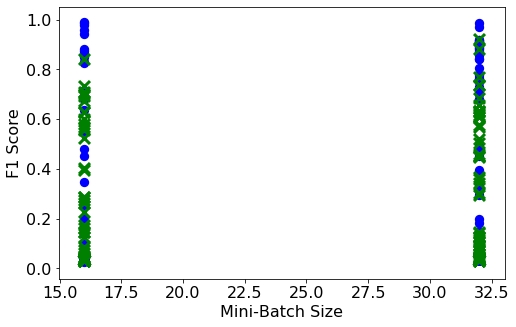
\includegraphics[width=\textwidth]{images/cnn_batch_size.png}
         \caption{}
         \label{fig:cnn_batch_size}
     \end{subfigure}
     \hfill
     \begin{subfigure}[b]{0.49\textwidth}
         \centering
         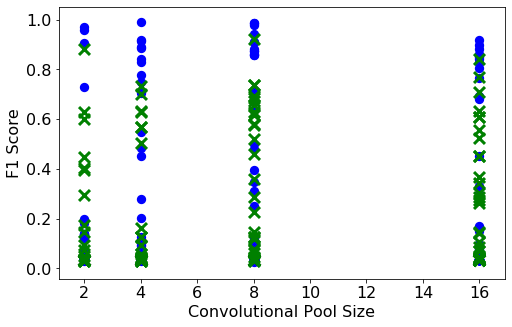
\includegraphics[width=\textwidth]{images/cnn_pooling_size.png}
         \caption{}
         \label{fig:cnn_pooling_size}
     \end{subfigure}

    \begin{subfigure}[b]{0.49\textwidth}
         \centering
         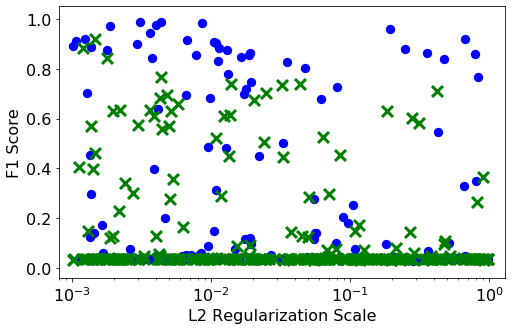
\includegraphics[width=\textwidth]{images/cnn_l2_reg.png}
         \caption{}
         \label{fig:cnn_l2_reg}
     \end{subfigure}
     \hfill
     \begin{subfigure}[b]{0.49\textwidth}
         \centering
         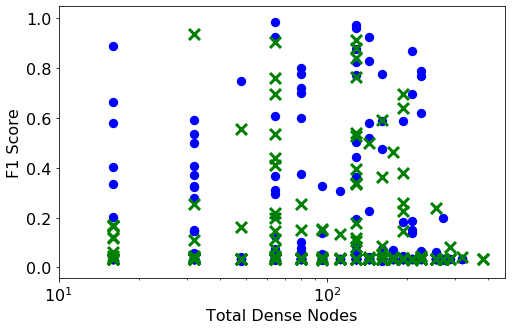
\includegraphics[width=\textwidth]{images/cnn_dense_nodes_total.png}
         \caption{}
         \label{fig:cnn_dense_nodes_total}
     \end{subfigure}  
     
     \begin{subfigure}[b]{0.49\textwidth}
         \centering
         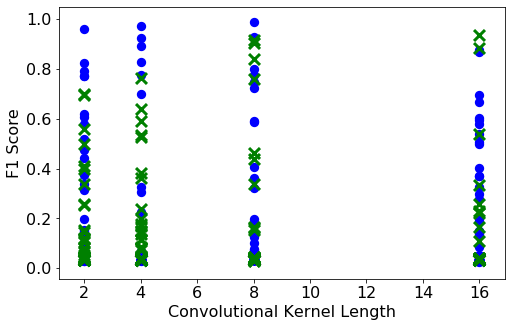
\includegraphics[width=\textwidth]{images/cnn_kernel_length.png}
         \caption{}
         \label{fig:cnn_kernel_length}
     \end{subfigure}
     \hfill
     \begin{subfigure}[b]{0.49\textwidth}
         \centering
         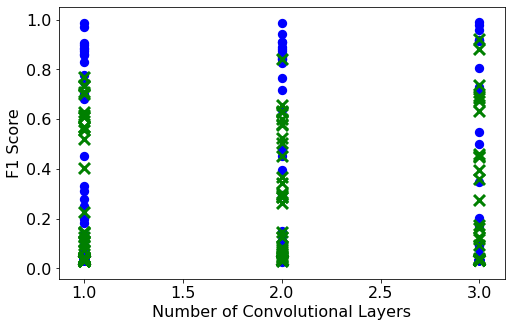
\includegraphics[width=\textwidth]{images/cnn_num_conv_layers.png}
         \caption{}
         \label{fig:cnn_num_conv_layers}
     \end{subfigure}  
	\begin{tabular}{r@{ : }l r@{ : }l}
		\textcolor{darkgreen}{\textbf{\large{X}}} & Complete Dataset & \bluecircle & Simple Dataset \\
	\end{tabular}
    \caption{Effect of CNN hyperparameters on the validation dataset's final F1 score.}
\end{figure}

\begin{figure} \ContinuedFloat
    \centering
    
    \begin{subfigure}[t]{0.49\textwidth}
        \centering
        % \raisebox{-0.49cm}{
        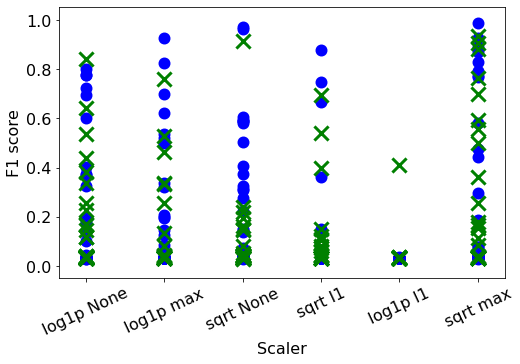
\includegraphics[width=\textwidth]{images/cnn_scaler.png}
        % }
        \caption{}
        \label{fig:cnn_scaler}
    \end{subfigure}
    \hfill
    \begin{subfigure}[t]{0.49\textwidth}
        \centering
        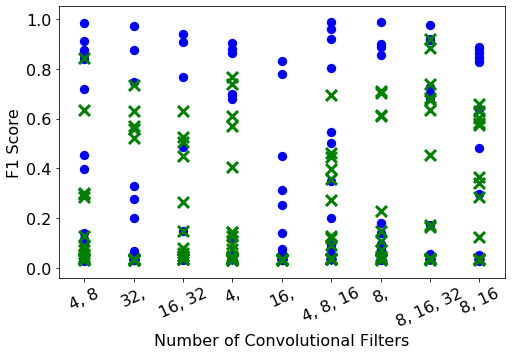
\includegraphics[width=\textwidth]{images/cnn_filter_structure.png}
        \caption{}
        \label{fig:cnn_filter_structure}
    \end{subfigure}
    
    \begin{subfigure}[t]{0.49\textwidth}
        \centering
        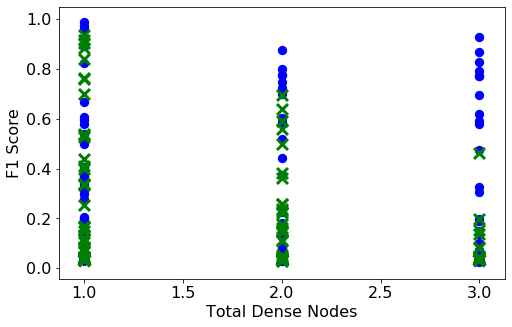
\includegraphics[width=\textwidth]{images/cnn_dense_layers_total.png}
        \caption{}
        \label{fig:cnn_dense_layers_total}
    \end{subfigure}
	\hfill
	\begin{subfigure}[t]{0.49\textwidth}
		\centering
		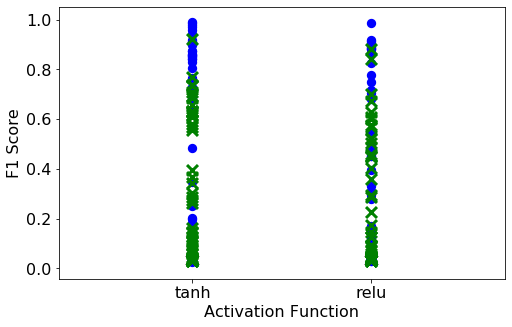
\includegraphics[width=\textwidth]{images/cnn_activation_function.png}
		\caption{}
		\label{fig:cnn_activation_function}
	\end{subfigure}

		\begin{tabular}{r@{ : }l r@{ : }l}
			\textcolor{darkgreen}{\textbf{\large{X}}} & Complete Dataset & \bluecircle & Simple Dataset \\
		\end{tabular}
        \caption{Effect of CNN hyperparameters on the validation dataset's final F1 score.}
        \label{fig:cnn_hyperparameters_f1_score}
\end{figure}

\begin{table}[H]
\centering
\caption{Optimum CNN hyperparameter combination found for the simple and complete dataset.}
\label{table:hyperparameter_opt_parameters_CNN}
\begin{tabular}{lll}
\hline
\multirow{2}{*}{\textbf{Hyperparameter}} & \multicolumn{2}{l}{\textbf{Optimum Value}} \\
 & \textbf{Simple Dataset} & \textbf{Complete Dataset} \\ \hline
Filter Kernels in Each Layer & 4 - 8 - 16 & 8 - 16 - 32 \\
Filter Kernel Length & 16 & 16 \\
Pooling size & 4 & 8 \\
Dense Layer Structure & 128 - 64 & 128 - 64 \\
Initial Learning Rate & 0.0014 & 0.00010 \\
L2 Regularization Strength & 0.0044 & 0.0015 \\
Dropout Frequency & 0.042 & 0.045 \\
Batch Size & 16 & 32 \\
Activation Function & tanh & tanh \\
Input Scaling & sqrt-max & sqrt-max \\ \hline
\end{tabular}
\end{table}

% \begin{table}[H]
% \centering
% \caption{Range of hyperparameters explored for the CNN.}
% \label{table:hyperparameter_dataset_parameters_CNN}
% \begin{tabular}{ccc}
% % \cline{2-3}
%  & Hyperparameter Range & Sampling \\ \hline
% \multicolumn{1}{c}{} & \begin{tabular}[c]{@{}c@{}}(4)   (8)   (16)    (32)\\ (4, 8)  (8, 16)  (16, 32)\\ (4, 8, 16)   (8, 16, 32)\end{tabular} & Uniform \\
% \multicolumn{1}{c}{} & 2, 4, 8, 16 & Uniform \\
% \multicolumn{1}{c}{} & 2, 4, 8, 16 & Uniform \\
% \multicolumn{1}{c}{} & 1 - 3 & Uniform \\
% \multicolumn{1}{c}{} & 10 - 1000 & Log-Uniform \\
% \multicolumn{1}{c}{} & 10$^{-4}$ - 10$^{-1}$ & Log-Uniform \\
% \multicolumn{1}{c}{} & 10$^{-3}$ - 10$^{0}$ & Log-Uniform \\
% \multicolumn{1}{c}{Dropout Frequency} & 0 - 1 & Uniform \\
% \multicolumn{1}{c}{Batch Size} & 2$^{4}$ - 2$^{6}$ & Power of Two \\
% \multicolumn{1}{c}{Activation Function} & tanh, relu & Uniform \\
% \multicolumn{1}{c}{Input Scaling} & \begin{tabular}[c]{@{}c@{}}sqrt, sqrt-max,\\sqrt-L1 Norm,\\ log1p-None, log1p-max,\\ log1p-L1 Norm\end{tabular} & Uniform \\
% \end{tabular}
% \end{table}

\subsection{Autoencoder Architectures} \label{section_autoencoder_archetectures}

Without an autoencoder, a single ANN has to learn multiple tasks to identify isotopes. An ANN would have to simultaneously identify the detector calibration, background signal, and source signal. By pretraining each network using an autoencoder to reconstruct a background-subtracted spectrum, the task of isotope identification is simplified for the ANN. To determine if using pretrained models results in more accurate identifications, a DAE and CAE were trained using the model parameters found in the hyperparameter search.

% (Tables \ref{table:hyperparameter_dataset_easy_parameters} and \ref{table:hyperparameter_dataset_full_parameters})
Pretraining was performed using a dataset of 10000 samples generated using the simple and complete dataset parameters. Because of the implicit regularization of the undercomplete encoding and the denoising background subtracting process, both networks do not use additional regularization when training. The initial learning rate of each autoencoder was set to 10$^{-5}$.

% This section will explain the hyperparameter structures searched. The autoencoder used is a undercomplete denoising autoencoder \cite{Goodfellow-et-al-2016}. Because the denoising operation performs regularization implicitly, no additional regularization is added to the autoencoders. 

% The autoencoder structures are found using a grid search. The autoencoders that reproduce the background subtracted signal the best are used in a dense random hyperparameter search as the signal preprocessing.


% The DAE structure is based on the dense hyperparameter search. The DAE trained on both datasets uses the same parameters as Table \ref{table:hyperparameter_dataset_parameters_DNN} without regularization and with an initial learning rate set to 10$^{-5}$. The DAE does not use L2 regularization or dropout due to the implicit regularization of the undercomplete encoding and the denoising background subtracting process.

% \begin{table}[H]
% \centering
% \caption{Optimum DNN hyperparameter combination found for the simple and complete dataset.}
% \label{table:hyperparameter_dataset_parameters_DNN}
% \begin{tabular}{ccc}
% \multirow{2}{*}{Hyperparameter} & \multicolumn{2}{c}{Optimum Value} \\
%  & Simple Dataset & Complete Dataset \\ \hline
% Dense Layer Structure & (64) & (32) \\
% Initial Learning Rate & 10$^{-5}$ & 10$^{-5}$ \\
% Batch Size & 256 & 16 \\
% Activation Function & relu & relu \\
% Input Scaling & sqrt & sqrt-max
% \end{tabular}
% \end{table}

% The CAE structure is based on the convolutional hyperparameter search. The CAE's trained on both datasets use the same parameters as Table \ref{table:hyperparameter_dataset_parameters_CNN} without regularization and with an initial learning rate set to 10$^{-5}$.


% \section{Summary of Final Model Architectures}


% This section discusses performance differences between the DNN, CNN, CAE-DNN, and DAE-DNN. These differences will be based on the final testing set error for all models.  





